
\section*{\centering Exponentiellt sönderfall}

\subsection*{Teori}

Detta avsnitt grundar sig på kapitel 31.8 och 40 i Tipler och Moscas bok \textit{Physics for Scientists and Engineers} (2008).

Efter att atomer har absorberat energi i form av elektromagnetisk (EM) strålning så emitterar de EM strålning tillbaka. Atomernas emission av EM strälning kallas fluorescens som är kortlivat för de flesta atomer. Antal emitterad fotoner (intensitet $I$) vid angiven tidspunkt $t$ ges av
\begin{equation} \label{eq:I_t}
	I(t) = I_0e^{-t/\tau},
\end{equation}
där $I_0$ är intensiteten då mätningen börjar ($t=0$) och $\tau$ är medellivslängden.

Vid högt antal detekterade fotoner så kan Poissonfördelning approximeras till normalfördelning och ger samma avvikelse $\sigma$ i mätningen av intensiteten.
\begin{equation} \label{eq:I_err}
    \sigma = \sqrt{I}
\end{equation}
Bra empirisk data av emissionsintensiteten ger bra underlag för att hitta tidskonstanten (medellivslängden) för givna atomer. Detta kan göras genom att skriva om ekvation~\ref{eq:I_t} som
\begin{equation} \label{eq:log_I}
	\text{ln}(I(t)) = -\dfrac{t}{\tau} + \text{ln}(I_0)
\end{equation}
och hitta $\tau$ (tidskonstanten) genom linjärisering;
\begin{align}
    k = -\dfrac{1}{\tau} 
    \quad &\Leftrightarrow \quad
	\tau = -\dfrac{1}{k} \label{eq:1_k},
	% b = \text{ln}(I_0) \quad &\Leftrightarrow \quad
	% I_0 = e^{b}
\end{align}
för att sedan beräkna halveringstid $t_{1/2}$ med
\begin{equation} \label{eq:halflife}
    t_{1/2}=\text{ln}(2)\tau.
\end{equation}

\subsection*{Resultat}
Figur~\ref{fig:1_1} presenterar data för observerat antal fotoner.
\begin{figure}[H]
    \centering
    \captionsetup{justification=centering,margin=2cm}
    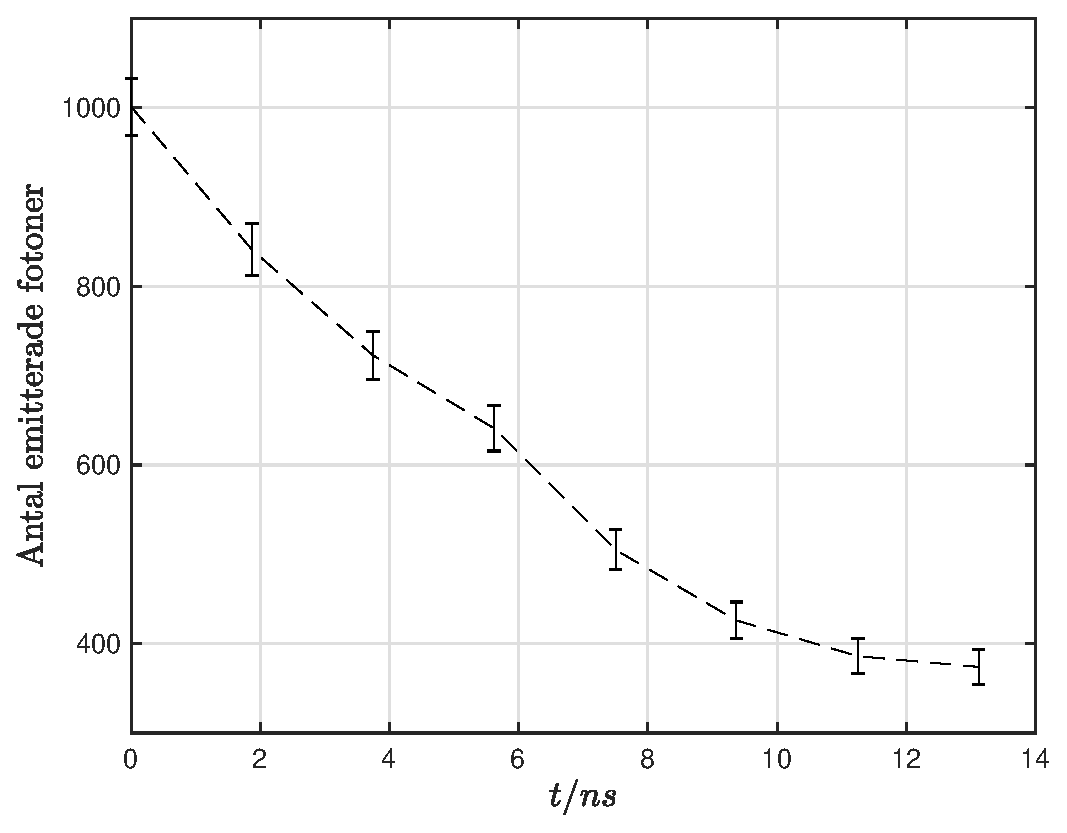
\includegraphics[scale=0.4]{Resources/Graphics/fig1_1.eps}
    \caption{Observerat antal emitterade fotoner inklusive osäkerhet i mätningar.}
    \label{fig:1_1}
\end{figure}

Från Figur~\ref{fig:1_2} beräknades medellivslängd $\tau$ med ekvation~\ref{eq:1_k} till 12.5 ns och halveringstid med ekvation~\ref{eq:halflife} till 8.66 ns. En modell för emissionsintensitet vid en viss tid skapades baserad på resultat och plottades i Figur~\ref{fig:1_3} med observerad data.
\begin{figure}[H]
    \minipage{0.47\textwidth}
        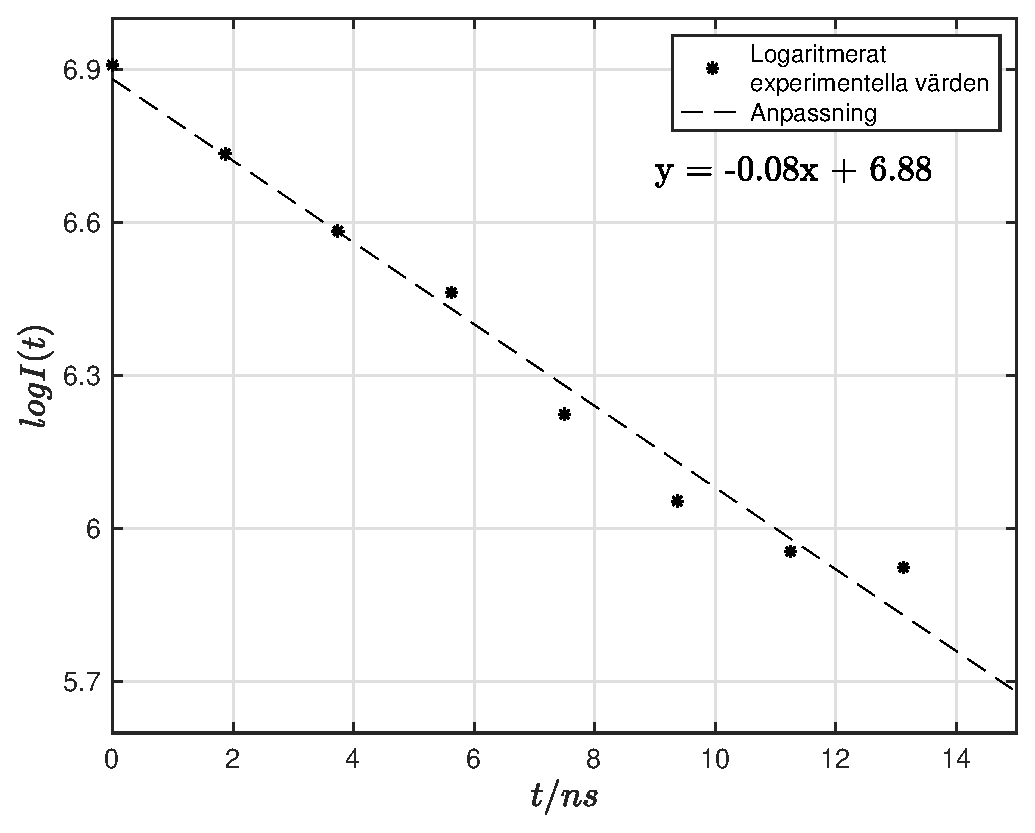
\includegraphics[width=\linewidth]{Resources/Graphics/fig1_2.eps}
        \caption{Linjärisering av data från Figur~\ref{fig:1_1}}\label{fig:1_2}
    \endminipage\hfill
    \minipage{0.47\textwidth}
        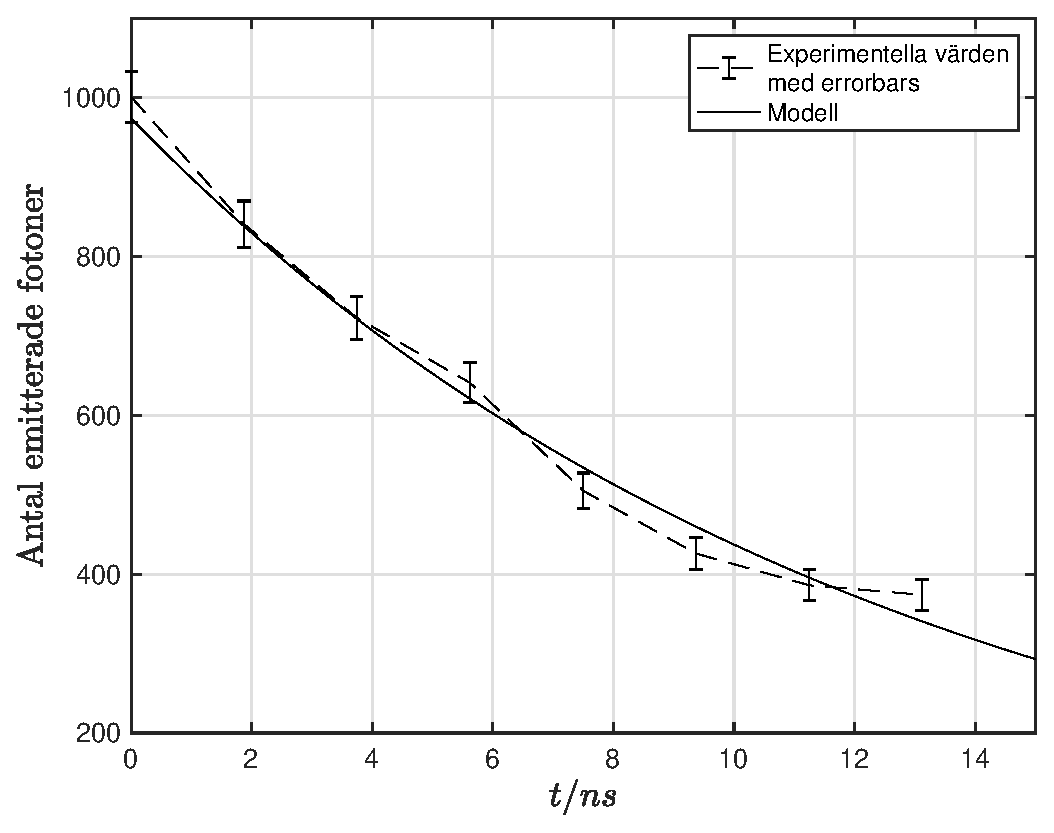
\includegraphics[width=\linewidth]{Resources/Graphics/fig1_3.eps}
        \caption{Observerad data och en modell för tidskonstanten}\label{fig:1_3}
    \endminipage
\end{figure}

\subsection*{Kommentar}
I figur~\ref{fig:1_3} syns det att osäkerhetsformeln $\pm\sqrt{I}$ stämmer bra för höga $I$, men dåligt för låga $I$. Detta kan förklaras med att Poissonfördelning ej bör approximeras till normalfördelning för lågt antal diskreta element.

\subsection*{Referenser}
Mosca, Gene; Tipler, A., Paul. 2008. \textit{Physics for Scientists and Engineers}. 6:e upplagan. W.H. Freeman and Company, New York.

\np
\subsection*{MatLab-kod}

% TODO: Latex doesn't like ä in Matlab code :/
% Change to English?
\lstinputlisting[caption={\quad},firstline=2] {Resources/Code/1.m}